\section{DERI - International}

DERI International is constituted of four research institutes. DERI Innsbruck,
located at the Leopold-Franzens University in Austria, and DERI Galway,
located at the National University of Ireland Galway in Ireland, are the two
founding members and key players. DERI Stanford and DERI Korea are
representative members of DERI in their country and are research institutes
that have joined DERI International. DERI performs academic research and leads
many projects in the Semantic Web and Semantic Web Service field. DERI has been
successfully acquiring large European research projects in the Semantic Web
area such as DIP\footnote{DIP: \url{http://dip.semanticweb.org/}} (Data,
Integration and Processes) or Nepomuk\footnote{Nepomuk:
\url{http://nepomuk.semanticdesktop.org}} (Semantic Web desktop). DERI
collaborates with several large industrial partners as HP, ILOG, IBM and CISCO
but also with medium-sized and small industrial enterprises. DERI is aware of
industry requirements and maintains close relationships with industrial
partners in order to validate research results and transfer them to industry.
DERI also has many research partners, such as the W3C, FZI Karlsruhe or \'Ecole
Polytechnique F\'ed\'erale de Lausanne (EPFL).

\section{DERI - Galway}

DERI Galway was founded in June 2003 by prof.dr. Dieter Fensel and is
currently managed by prof.dr. Stefan Decker. DERI Galway is attached to the
National University of Ireland Galway (NUIG). DERI Galway currently has 130
members composed of senior researchers, PhD students, master and bachelor
students, management staffs and interns. DERI is a Centre for Science and
Engineering Technology (CSET) funded principally by the Science Foundation
Ireland (SFI) but also by Enterprise Ireland, the Information Society
Technologies (EU) and the Irish Research Council for the Humanities and Social
Sciences. DERI divides its research into three main domains
\begin{enumerate}
  \item Social Semantic Information Spaces
  \item Semantic Reality
  \item Application Oriented Research Domain
\end{enumerate}
Within these research strands individual units focus on one core competency
for realising DERI’s mission and its work with its industrial partners. Each
unit specialises in a particular research discipline that has relevance for
realising the overall goals of the institute.

\section{The Mission}

The Web is an area in constant progress, and a major step is on its way:
linking together the real work with the virtual world. A first revolution was
done with the apparition of social networking. This marked an important change
in the way people have been using the Internet: a massive amount of data are
now available and shared. Individuals as well as enterprises gain from it.
However the use of this data is limited because they are platform specific
(e.g. LinkedIn, Facebook, Myspace, \ldots). There are \emph{islands of
information} that do not link to each other.

DERI's mission is to research new technologies that will realise the link
between the real and the virtual worlds (Figure~\ref{fig:deri-mission}): the
development of applications using the semantics of data, software that
inter-connects the islands of information. Two main steps are necessary to
achieve this link:
\begin{enumerate}
  \item \emph{sensors} that collect data from the physical world:
  temperature sensors for home automation, body sensors such as the heartbeats
  to better help people control their health.
  \item \emph{semantic spaces} that break down barriers between information
  allowing their thorough use.
\end{enumerate}
These axes lead to the realisation of linking the real world with the virtual
world, creating what DERI calls the \emph{semantic
reality}~\cite{decker:2008:semantic-reality}.

\begin{figure}
\centering
\resizebox{0.6\linewidth}{!}{%
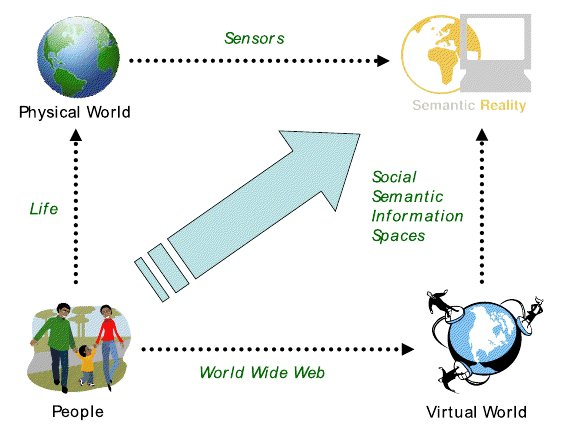
\includegraphics[scale=1]{pics/deri-mission}
}
\caption{Semantic reality.}
\label{fig:deri-mission}
\end{figure}

\subsection{DI2 - Data Intensive Infrastructures}

DI2 position itself within DERI as a unit which purpose is to develop systems
and infrastructures in order to make Social Semantic Spaces a possibility.
The requirements to analyse and understand the inner workings and underlying
fundamental concepts of the Web along with the elevated scalability
requirements for the development of new Web infrastructures have demonstrated
the necessity of Data Intensive Supercomputing (DISC) infrastructures to
support researchers and developers. A prominent characteristic of DISC (as
promoted by major players such as Google, Yahoo and MSN), as opposed to
classic supercomputing, is the importance of very advanced data management
software over high-end hardware configurations. DISC data entries are in fact
known to be formed by hundreds or thousands of commodity machines connected
using common commercial networking infrastructures. It is then up to the
software to be able to deliver high capacity, throughput, scalability,
re-configurability and fault tolerance. To be able to conduct credible
research and development in the Web domain, DERI requires a DISC
infrastructure. As DISC in itself is the subject of ongoing research, the goal
of this work programme is to advance the research and applications of data
intensive infrastructures, to create, maintain and offer to researchers a
state-of-the-art DISC infrastructure, and to research novel algorithms and
data structures for scalable handling of large amounts of semantic
information.

\section{Working Environment}

My internship lasted from February 2010 to December 2010 within the Data
Intensive Infrastructures (DI2) unit. \emph{Sig.ma} is a semantic web
application based on Sindice, the web service that provides search and
retrieval capabilities over semantic data. At the core Sindice uses SIREn, a
search engine based on Information Retrieval, for the purpose of retrieving
semantic data. My supervisors were Renaud Delbru, Ph.D student at the time but
graduated to doctor on December, and Dr. Giovanni Tummarello. The internship
consisted  to assist Renaud Delbru on his thesis about SIREn.

My work was closely watched by my supervisors, with a regular meeting between
R.Delbru and myself in order to discuss the progress, new research ideas,
design and implementations. The research was performed based on other research
scientific publications, in order to provide a solid background for our own
research.

On the hardware aspect, DERI lent me a laptop for the duration of the
internship. Also I had access to DERI servers so that I could perform my own
experiments and benchmarks on a sane environment.

As for the programming languages used during the internship, JAVA and scripting
languages such as shell scripts, ruby, python and sed were used.

